\documentclass[12pt]{gatech-thesis}
\usepackage{amsmath,amssymb,latexsym,float,epsfig,subfigure}
\usepackage{booktabs}
\usepackage{multirow}
\usepackage{siunitx}
%\usepackage[round]{natbib}




%%
%% This example is adapted from ucthesis.tex, a part of the
%% UCTHESIS class package...
%%
\title{People Aware Mobile Robot Navigation} %% If you want to specify a linebreak
                               %% in the thesis title, you MUST use
                               %% \protect\\ instead of \\, as \\ is a
                               %% fragile command that \MakeUpperCase
                               %% will break!
\author{Akansel Cosgun}
\department{College of Computing}

%% Can have up to six readers, plus principaladvisor and
%% committeechair. All have the form
%%
%%  \reader{Name}[Department][Institution]
%%
%% The second and third arguments are optional, but if you wish to
%% supply the third, you must supply the second. Department defaults
%% to the department defined above and Institution defaults to Georgia
%% Institute of Technology.

\principaladvisor{Professor Henrik Christensen}
\committeechair{Professor Ignatius Arrogant}
\firstreader{Professor General Reference}[School of Mathematics]
\secondreader{Professor Ivory Insular}[Department of Computer Science and Operations Research][North Dakota State University]
\thirdreader{Professor Earl Grey}
\fourthreader{Professor John Smith}
\fifthreader{Professor Jane Doe}[Another Department With a Long Name][Another Institution]
%\setcounter{secnumdepth}{2}
\degree{Doctor of Philosophy}

%% Set \listmajortrue below, then uncomment and set this for
%% interdisciplinary PhD programs so that the title page says
%% ``[degree] in [major]'' and puts the department at the bottom of
%% the page, rather than saying ``[degree] in the [department]''

%% \major{Algorithms, Combinatorics, and Optimization} 

\copyrightyear{2010} 
\submitdate{August 2010} % Must be the month and year of graduation,
                         % not thesis approval! As of 2010, this means
                         % this text must be May, August, or December
                         % followed by the year.

%% The date the last committee member signs the thesis form. Printed
%% on the approval page.
\approveddate{1 July 2010}


\bibfiles{example-thesis}

%% The following are the defaults
%%    \titlepagetrue
%%    \signaturepagetrue
%%    \copyrightfalse
%%    \figurespagetrue
%%    \tablespagetrue
%%    \contentspagetrue
%%    \dedicationheadingfalse
%%    \bibpagetrue
%%    \thesisproposalfalse
%%    \strictmarginstrue
%%    \dissertationfalse
%%    \listmajorfalse
%%    \multivolumefalse

\begin{document}
%\bibliographystyle{plainnat}
\bibliographystyle{gatech-thesis}
%%
\begin{preliminary}
\begin{dedication}
\null\vfil
{\large
\begin{center}
To myself,\\\vspace{12pt}
Perry H. Disdainful,\\\vspace{12pt}
the only person worthy of my company.
\end{center}}
\vfil\null
\end{dedication}
\begin{preface}
Theses have elements.  Isn't that nice?
\end{preface}
\begin{acknowledgements}
I want to thank people
\end{acknowledgements}
% print table of contents, figures and tables here.
\contents
% if you need a "List of Symbols or Abbreviations" look into
% gatech-thesis-gloss.sty.
\begin{summary}
Why should I provide a summary?  Just read the thesis.
\end{summary}
\end{preliminary}
%%
\chapter{Introduction}

Introduction

%%%%%%%%%%%%%%%%%%%%%%%%%%%%%%%%%%%%%%%%%%%%%

\chapter{Map Annotation}

Map Annotation
  
\section{Related Work}

Related Work

\section{Semantic Maps}

Semantic Maps

\subsection{Waypoints}

\subsection{Planar Landmarks}

\subsection{Objects}


\section{User Interface}

User Interface


\section{Pointing Gestures for Human-Robot Interaction}

Pointing Gestures

%%%%%%%%%%%%%%%%%%%%%%%%%%%%%%%%%%%%%%%%%%%%%

\chapter{Navigation Among People}

Autonomous Robot Navigation

\section{Related Work}

Related Work

\section{State of Autonomous Robot Navigation}

State of Autonomous Robot Navigation

\section{Finding Goal Points for Navigation}

Finding Goal Points for Navigation

\section{People Aware Navigation}

People Aware Navigation

\section{Speed Maps for Safe Navigation}

Speed Maps for Safer Navigation


%%%%%%%%%%%%%%%%%%%%%%%%%%%%%%%%%%%%%%%%%%%%%

\chapter{Multimodal Person Detection and Tracking}
\label{sec:multimodal_person_detection_and_tracking}
The ability to robustly track a person is an important prerequisite for human-robot interaction. To realize any task that involves humans, the challenge is the detection and tracking of humans in the vicinity of the robot considering the robot's movements, sensing capabilities and occlusions. The scope of how much information is needed from the human perception module depends on the objective of the application. First, the robot should determine if there are people nearby. If the robot senses people around, the robot should find out \emph{where} they are. Representing people as points (x,y) in maps is common practice for navigation planning. If the task requires the robot to face a person, then the orientation $\theta$ needs be detected. The robot further can determine \emph{who} the detected person is. Identification of humans is necessary for enabling non-generic service. Finally, the robot should interpret \emph{what} the person is doing by analyzing the motion features and through gesture analysis. Tracking body parts of humans over time give significant information about human activity.

We focus on tracking people who are either walking or standing, as these are the two most common human poses around a mobile robot. Many full-body or body part detectors have been developed in the literature, reviewed in Section~\ref{sec:multimodal_related_work}. Full-body detectors are not suitable for mobile robot navigation applications because of their inability of capturing the entire body with on-board sensors when people are close to the robot. We aim to robustly track a person $360^{\circ}$ around the robot. However, most sensors have a limited field of view and using only a single detector can lead to a system with a single point of failure. Therefore, we think a multimodal detection system is better suited for on-board people tracking for our use cases. 


Laser scanners are the natural sensor of choice as state-of-the-art mobile robots are already equipped with an ankle-height laser scanner that is mainly used for navigation. The laser scanners we used on our robot are Hokuyo UTM 30-LX, which has $270^{\circ}$ Field of View (FOV), $0.25^{\circ}$ angular resolution, $40Hz$ refresh rate and $30m$ maximum range. We are only interested in detections in close range (less than $5m$). In that range interval, and the accuracy of each laser reading is $\pm 3cm$, which is sufficient for our use cases. The relatively higher accuracy and resolution are the two advantages of laser scanners over cameras and RGB-D cameras. Cameras, on the other hand, have the advantage of providing richer information, which can be used to extract body parts. We use a combination of detectors using either a laser scanner and RGB-D camera for robustness and better coverage, described in Section~\ref{sec:multimodal_person_detection}. Representing people as a points in the map is sufficient for mobile robot navigation and each detector produces a point as a person hypothesis. We use a real-time probabilistic tracking framework that relies on the fusion of the multiple person detections, described in Section~\ref{sec:multimodal_person_tracking}. For certain applications, identifying specific users allows the robot to go beyond generic capabilities. We present our face recognition method in Section~\ref{sec:multimodal_face_recognition}.

\section{Related Work}
\label{sec:multimodal_related_work}

Person detection was first addressed by the computer vision community as an object detection problem. Early research on person detection using vision is surveyed by Moeslund \cite{moeslund2001}. Face detection is a common method for detecting people, with the work of Viola and Jones \cite{viola2004robust} being the most popular one. See Zhang \cite{zhang2010survey} for a survey on contemporary approaches on vision based face detection. Another popular topic has been pedestrian detection in crowded scenes Leibe \cite{leibe2005pedestrian} and Tuzel \cite{tuzel2007human}.

In 2000's, laser scanners became the de-facto sensor for localization and mapping. Laser scanners are usually placed slightly above floor for obstacle avoidance, therefore leg detection is common practice. Early works by Montemerlo \cite{montemerlo2002conditional} and Schulz \cite{schulz2001tracking} focused on tracking multiple legs using particle filters. Legs are typically distinguished in laser scans using geometric features such as arcs \cite{xavier2005fast} and boosting can be used to train a classifier on a multitude of features \cite{arras2007using}. Topp \cite{topp2005tracking} demonstrates that leg tracking in cluttered environments is prone to false positives. For more robust tracking, some efforts fused information from multiple lasers such as Carballo's work \cite{Carballo2008}, which uses a second laser scanner at torso level. Glas \cite{glas2009laser} uses a network of laser sensors at torso height in hall-type environments to track the position and body orientation of multiple people. Several works used different modalities of sensors to further improve the robustness. Kleinehagenbrock \cite{kleinehagenbrock2002person} and Bellotto \cite{bellotto2009multisensor} combine leg detection and face tracking in a multi-modal tracking framework. Other examples include combining sound localization and vision \cite{bernardin2007audio} and combining RFID tracking and vision \cite{germa2010vision}.

Laser-based person methods pertains tracking of humans in 2D, projected to floor plane. Tracking of the body parts has long been a topic of interest in vision \cite{baumberg1997learning,sidenbladh2000stochastic}. With the recent introduction of 3D sensors such as the Velodyne, Swissranger and Kinect, more robust tracking became possible. Spinello \cite{spinello2010layered} trains geometrical features at different height levels in the 3D point cloud for pedestrian detection. Ganapathi \cite{ganapathi2010real} estimates body part locations with a probabilistic model. One of the well-known skeleton tracking algorithms is the Microsoft Kinect SDK by Shotton \cite{shotton2013real}, which trains decision forests using simple depth features in a vast database. This software is not suitable to work on a mobile robot as it is designed to work on a stationary sensor. In the robotics community, there are efforts to develop skeleton trackers that work on mobile robots and in unstructured scenes \cite{buys2013adaptable}.

Face recognition is a widely used application as surveyed by Phillips \cite{phillips2005overview}. One of the pioneers in face recognition uses a set of patch masks for features that doesn't necessarily correspond to eyes, ears or noses \cite{turk1991face}. \cite{zhao1998discriminant} combines PCA (Principal Component Analysis) and LDA (Linear Discriminant Analysis) to improve the generalization capability when only a few samples are available.

There has been some work to identify humans using 3D data, such as the head-to-shoulder signature \cite{kirchner2012head} and body motion characteristics \cite{munsell2012person}. Biometric person identification techniques, such speaker recognition \cite{kinnunen2010overview}, 3D ear shape \cite{yan2007biometric} and multi-modal cues \cite{garcia2003biomet} have potential to be more accurate than face recognition. However, these approaches are better suited to work in controlled environments.

\section{Person Detection}
\label{sec:multimodal_person_detection}

In this section, we present our person detectors, namely leg detection (Section \ref{sec:multimodal_leg_detection}) and torso detection (Section \ref{sec:multimodal_torso_detection}). We also use an implementation of an upper body detector by Mitzel \cite{mitzel2012close}, which uses a template and the depth information of a RGB-D camera to identify upper bodies (shoulders and head), designed to work for close range human detection using head mounted cameras.

\subsection{Leg Detection}
\label{sec:multimodal_leg_detection}

A front-facing laser scanner at ankle height is used for leg detection. The output of a laser scanner at each iteration is an array of range measurements, represented in the polar coordinate system. We first convert the range data to Cartesian coordinate system:

\[
x_{i} = \sum_{\phi = \phi_{start}}^{\phi_{end}} r_i\cos(\phi)
\]
\[
y_{i} = \sum_{\phi = \phi_{start}}^{\phi_{end}} r_i\sin(\phi)
\]

Then we apply segmentation, Segmentation produces clusters of consecutive scan points, which due to their proximity, have a high likelihood of belonging the same object. Two adjacent distance measurements are considered to be in the same segment if the Euclidean distance between them is below a threshold value. Starting from the start of the range array, a new segment is started if $|r_{i}-r_{i+1}|<d_{cluster}$. Although some approaches use a variable segmentation threshold that is a function of the range, we use a fixed clustering threshold $d_{cluster}=0.1m$. The segmentation process results in a set of segments $\mathbf{S}$. A set of geometric features are extracted from the laser segment.

In a laser scan, legs can appear in different patterns \cite{topp2005tracking}. We look only single leg and person-wide blob patterns as these two cover all the ways legs can be seen in a laser scan. Depending on the application, we accept either only the single leg pattern or both of the patterns (explained in Section \ref{sec:multimodal_person_tracking}.

There are a number of geometric features that can be extracted from a laser segment, as delineated by Arras \cite{arras2007using}. We use three geometric features that is used to detect a leg: segment width, circularity, and Inscribed Angle Variance (IAV):


\begin{enumerate}
\item Segment Width: Measures the Euclidean distance between the first and last point of a segment $S_i$




\item Segment Circularity: This measure is a simple measure to assess if the segment shape resembles a circle. The circularity criterion we used is the ratio of the perpendicular distance from the middle point to the line segment that connects start and end points, to the segment width. For example, in a perfect half circle in Figure \ref{fig:circ1}, the circularity criterion is $|\overline{P_0P_n}/d_{mid}=0.5$. In case of a laser scan, as can be seen in Figure \ref{fig:circ2}, we again consider the ratio of $d_{mid}$ to segment width. For this calculation we only consider the middle point as it provides a simple heuristic on circularity.

\begin{figure}[ht!]
  \centering
  \begin{minipage}[b]{0.49\textwidth}
    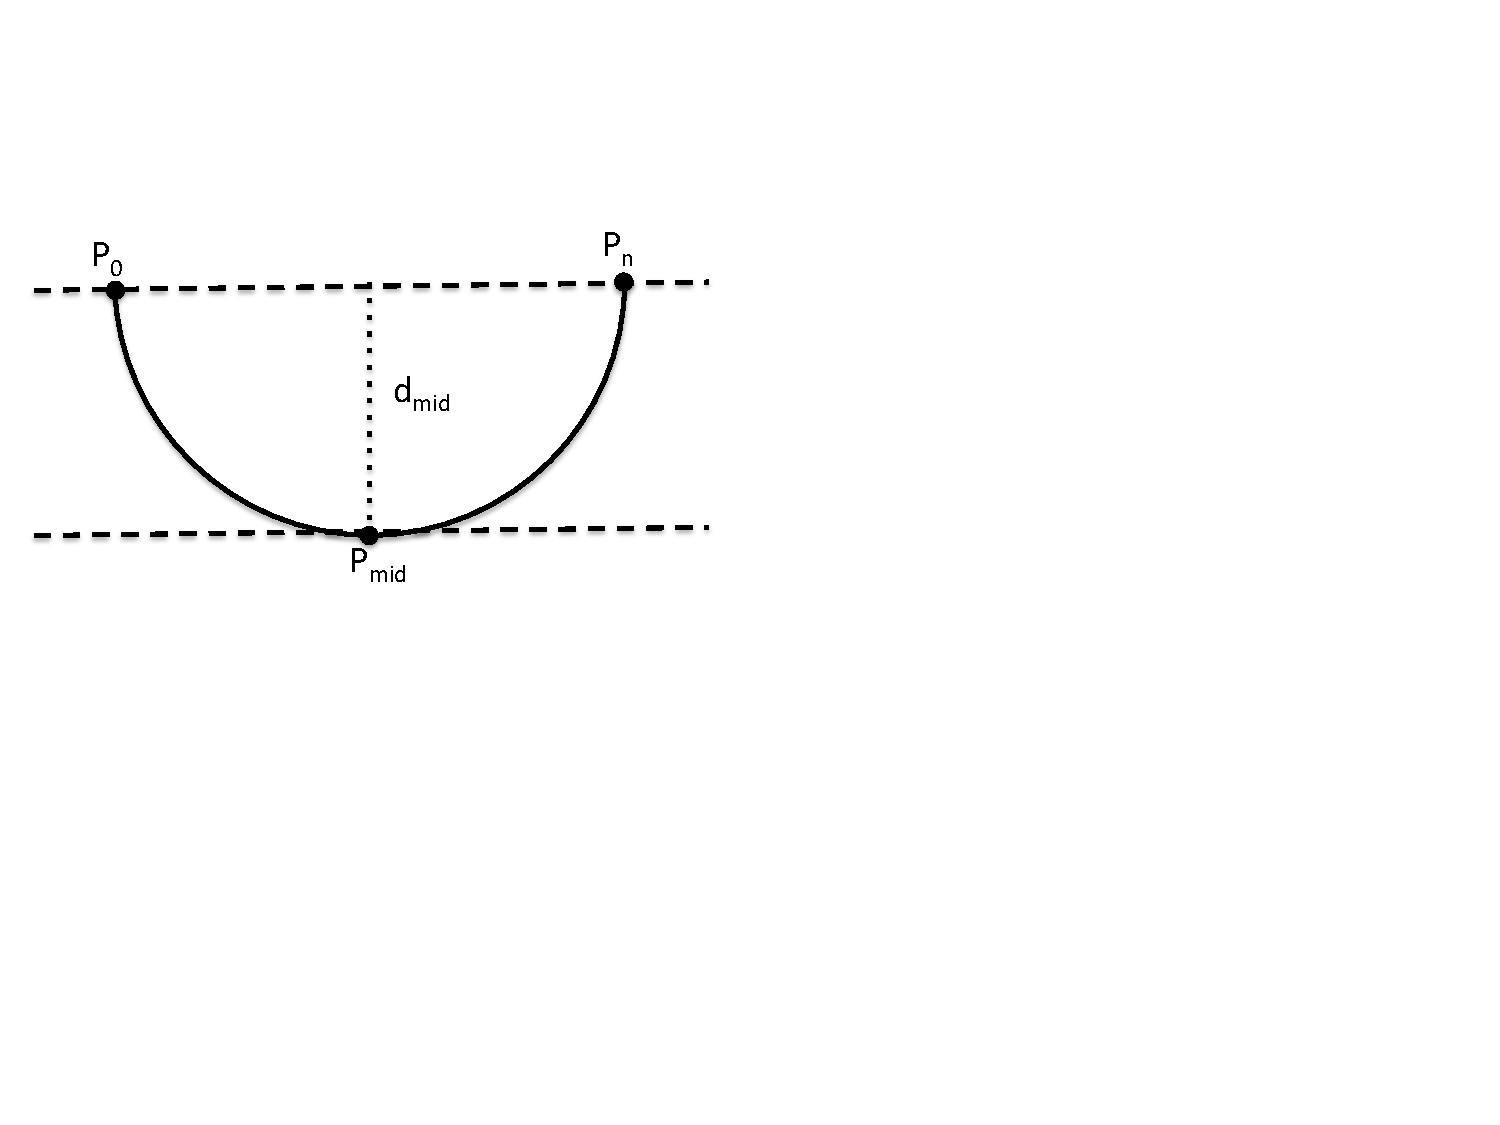
\includegraphics[width=\textwidth]{pics/circ1}   
    \caption{Circularity criterion in a perfect circle is: $|P_0P_n|d_{mid}=0.5$}
     \label{fig:circ1}
  \end{minipage}
  \hfill
  \begin{minipage}[b]{0.49\textwidth}
    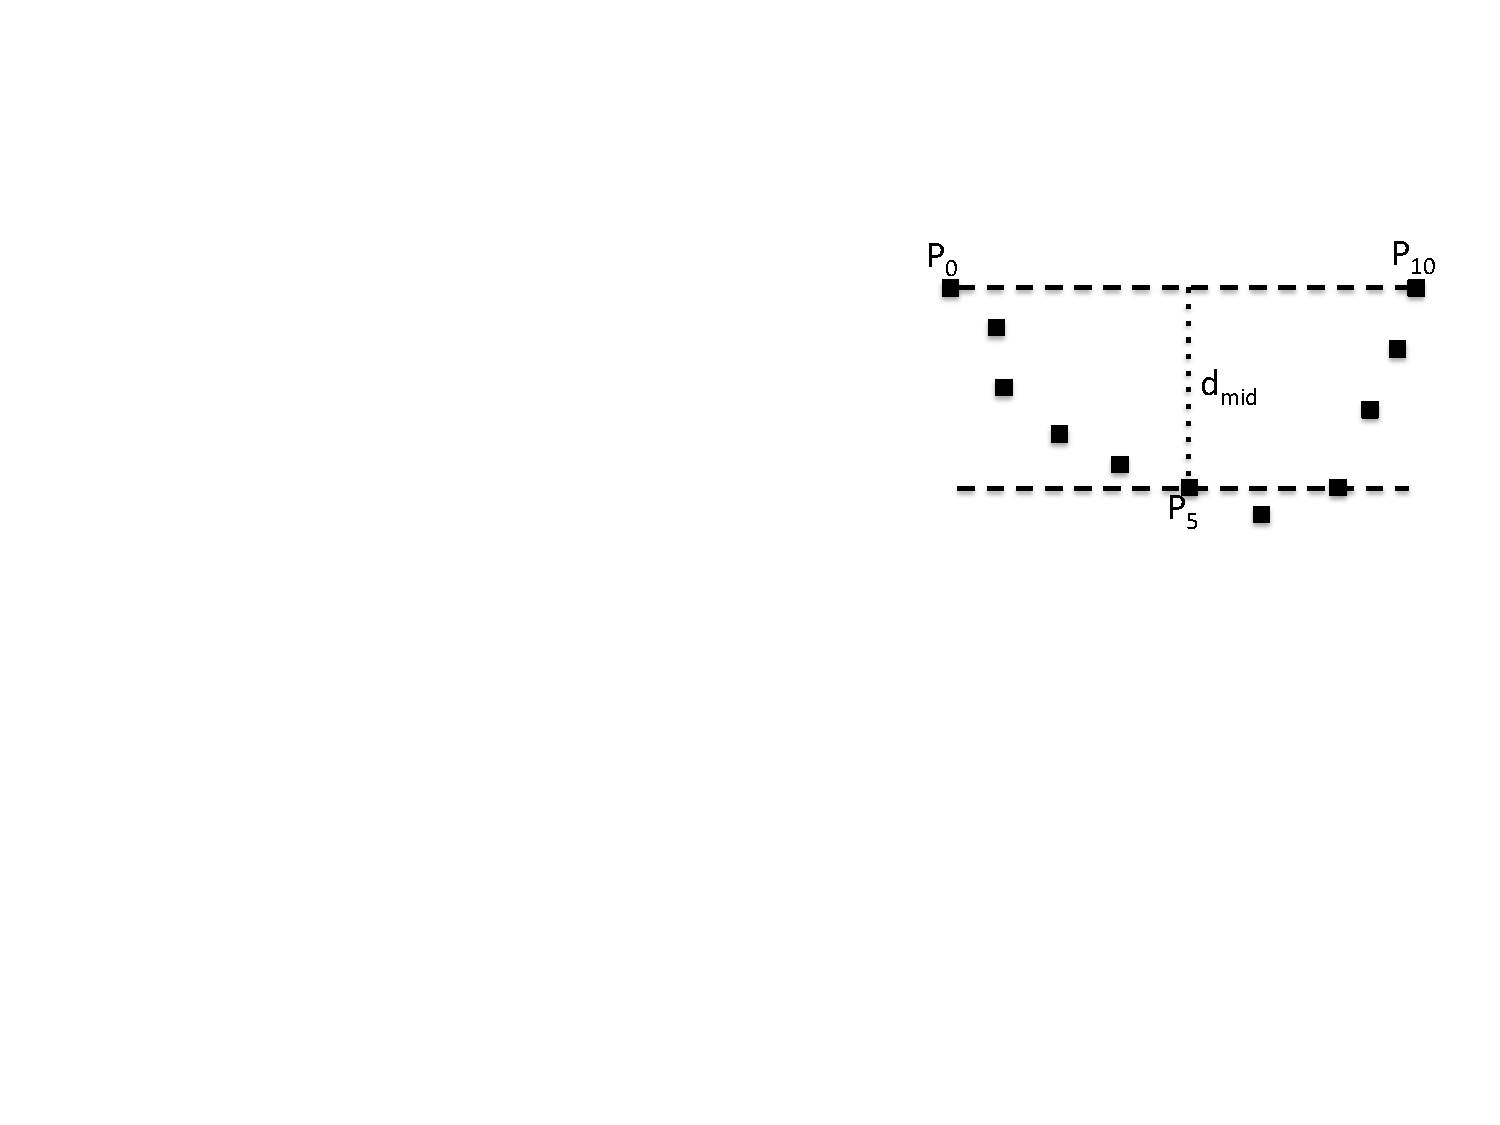
\includegraphics[width=\textwidth]{pics/circ2}    
    \caption{Circularity criterion in a this laser segment is: $|P_0P_{10}|/d_{mid}$}
    \label{fig:circ2}
  \end{minipage}
\end{figure}

\item Inscribed Angle Variance (IAV): This feature is originally proposed by Xavier \cite{xavier2005fast}, in order to detect circles. We adopt IAV in order to detect legs, which are not necessarily circle-shaped, especially for the person-wide blob pattern. As an example, inscribed angles on a circle is shown in Figure \ref{fig:iav}. As a geometric property of the circle, $\angle P_0P_1P_4$ and $\angle P_0P_2P_4$ are equal angles. IAV for a given set of points is the average of all inscribed angles: 

\[
IAV_S = \sum_{P = P_1}^{P_{n-1}} \angle P_0PP_n
\]



For a perfect circle, $IAV_S=90^{\circ}$. For shapes that are not perfect circles but are similar to circles, IAV feature should be consistent. Laser segments from a leg usually resemble a circle, therefore we use IAV as one of the features for leg detection.

\begin{figure}[ht!]
\centering
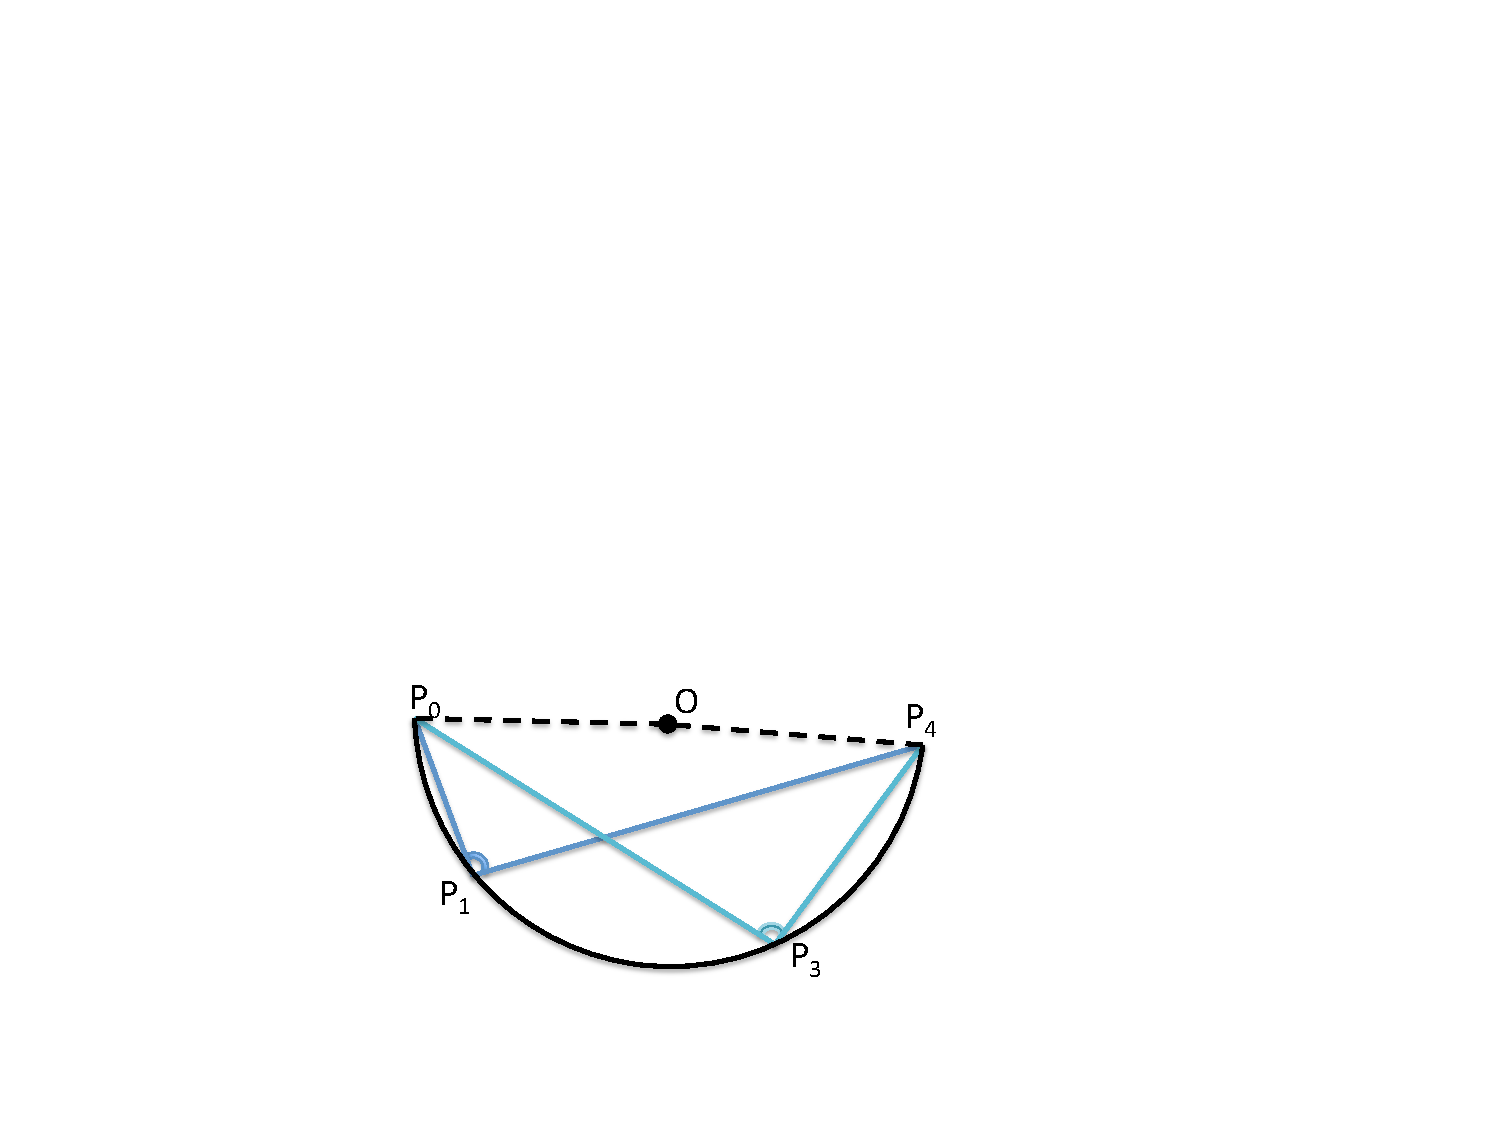
\includegraphics[width=0.4\textwidth]{pics/iav}
\caption{Inscribed angles of an arc are shown in the figure. Inscribed Angle Variance (IAV) is calculated by taking the average of all inscribed angles on a laser segment.}
\label{fig:iav}
\end{figure}

\end{enumerate}

In order to be able to use these values, we first found the nominal feature values for an average human leg. We captured the laser scan data while the robot followed a person through an office environment. The following method used for this experiment will be discussed in detail in Section \ref{sec:following_basic_person_following}. For the training set, two people's legs were recorded with different clothing (shorts, baggy pants and trousers) to account for variance in the leg parameters. About $17\times 10^3$ Single Leg patterns and $0.6\times 10^3$ person-wide blobs were manually labeled in the data. In addition, $120\times 10^3$ segments were labeled as 'other' or 'not a leg'. The average and variance of the aforementioned geometric features for single leg, personwide blob, as well as other segments are given in Table \ref{table:leg_features}. 

\begin{table}
	\centering
  \begin{tabular}{lSSSSSS}    
    \toprule
    \multirow{2}{*}{Segment type} &
      \multicolumn{2}{c}{Width($m$)} &
      \multicolumn{2}{c}{Circularity} &
      \multicolumn{2}{c}{IAV($radians$)} \\
      & {$\mu$} & {$\sigma$} & {$\mu$} & {$\sigma$} & {$\mu$} & {$\sigma$} \\
      \midrule
    Single Leg & 0.13 & 0.03 & 0.25 & 0.15 & 2.23 & 0.4 \\
    Personwide blob & 0.33 & 0.07 & 0.14 & 0.09 & 2.61 & 0.16 \\
    Other & 0.22 & 0.12 & 0.1 & 0.11 & 2.71 & 0.38 \\
    \bottomrule
  \end{tabular}
      \caption{Table shows average and standard deviations of geometric leg features calculated in our dataset.}
    \label{table:leg_features}
\end{table}

For every segment $S_i$ in a test laser scan, we first extract the geometric features $f_1^i,f_2^i,f_3^i$. We then calculate the weighted Mahalanobis distance to the average leg parameters for the each leg pattern:

\[
D_{mah}^i=\sum_{j=1}^3 k_j \frac{(f_j^i-\mu_j)^2}{\sigma_j^2}
\]

where $k_j$ are the weights for each feature, $mu_j$ and $sigma_j$ are pulled from Table \ref{table:leg_features}. The resulting Mahalanobis distance is then compared with a detection threshold. If $D_{mah}^i< d_{leg}$, the segment is considered a detection. 

\subsubsection{Associating Leg Segments}

After single leg patterns are detected, we try match the leg segments. We extend our leg detection approach to determine which leg segments are connected. Note that this method applies if there is a RGB-D camera pointing to the lower body of the human. For each leg segment pair, if both of them are within the FOV of the RGB-D sensor, we use our algorithm to determine whether there is a connectivity between two candidate leg segments. If a connectivity is found, then the leg segments pair is qualified to be a leg segment pair representing a person. See Figure \ref{fig:leg_connectivity} as an example result. Figure \ref{fig:leg_connectivity_diagram} shows the flow chart of the association algorithm.

\begin{figure}[ht!]
\centering
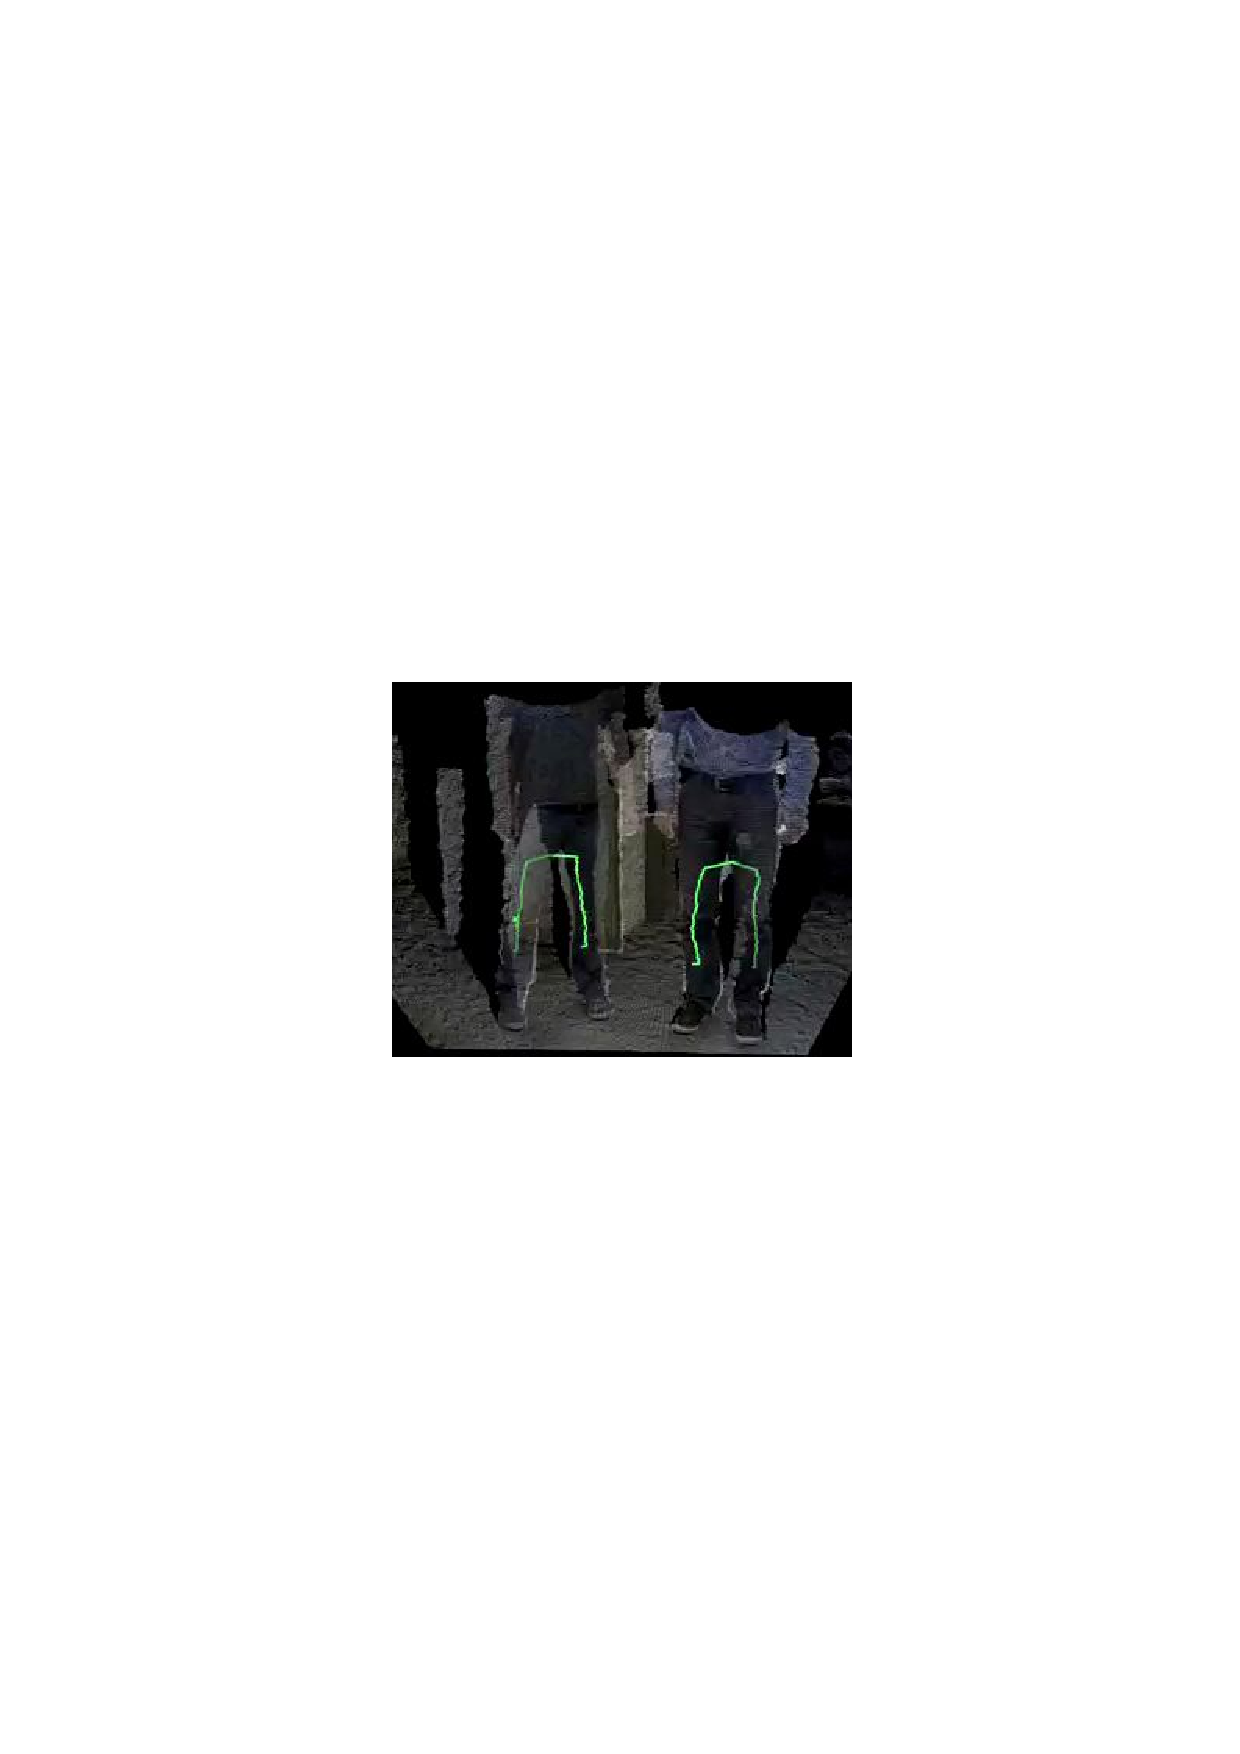
\includegraphics[width=0.6\textwidth]{pics/leg_connectivity}
\caption{Two person detections are seen in this figure. Our leg segment association algorithm propagates pixels vertically from candidate leg segments and connects leg pairs.}
\label{fig:leg_connectivity}
\end{figure}

\begin{figure}[ht!]
\centering
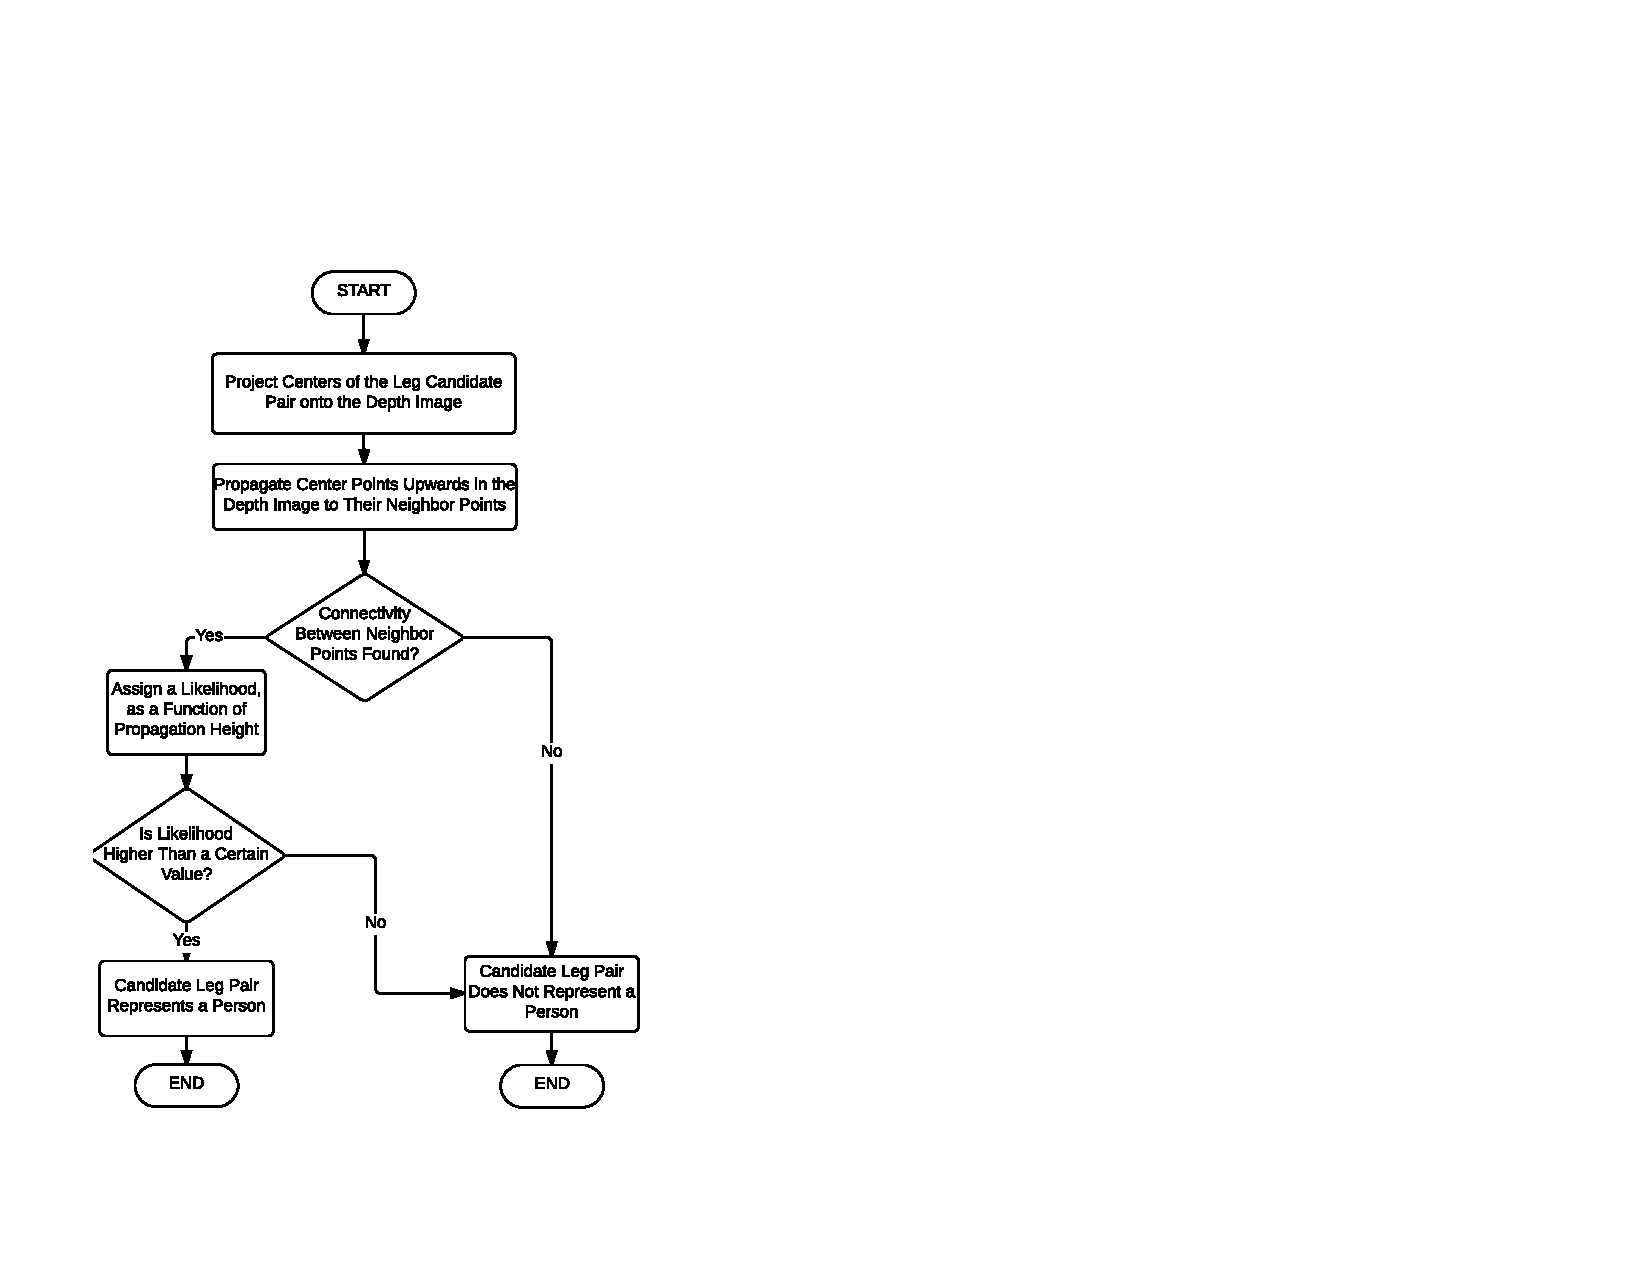
\includegraphics[width=0.5\textwidth]{pics/leg_connectivity_diagram}
\caption{Flow chart for determining if two leg segment candidates belong to a person.}
\label{fig:leg_connectivity_diagram}
\end{figure}

First, the centroids each of the two candidate leg segments are found.  These points are projected onto the depth image acquired from the RGB-D camera. At each iteration, each leg segment, our algorithm first propagates horizontally to both directions in the depth image, then the center pixel is located and it propagates 1 pixel vertically ($+z$ direction). If there are no connectivity after a number of iterations, then we conclude that the candidate leg pair does not represent a person. If there is a connectivity at some point, we then assign a likelihood score to the pair as a function of the vertical propagation height. If this score is higher than a threshold, then the algorithm concludes that the leg candidate segments represent a person. The propagation scoring eliminates most of the false positives due to sensor noise and non-human shapes.

\subsection{Torso Detection}
\label{sec:multimodal_torso_detection}

In this section, we describe our torso detection approach. For this detector, we used another Hokuyo UTM 30-LX laser scanner, placed at torso height ($1.27m$). Our approach relies on fitting an ellipse to laser segments and determining the detection result by interpreting the axis lengths. Our torso detector allows us to detect the orientation of the person unlike the laser-based leg detectors, therefore this detector is also suitable for applications that relies on extracting the orientation of the person from a single laser scan.

The first step to detect torsos in a laser scan is to segment the laser scan. We use the same segmentation technique used for leg detection, explained in Section \ref{sec:multimodal_leg_detection}. We then fit an ellipse to each laser segment. We use the ellipse fitting method proposed by 



\section{Person Tracking}
\label{sec:multimodal_person_tracking}

Multimodal Person Tracking

\section{Face Recognition}
\label{sec:multimodal_face_recognition}

Face Recognition

%A possible use of person recognition in interactive navigation is to drive up to a specific person. Another possible use case for our work is to re-initialize person following if the user is lost. We have used face recognition in some of our applications, however it requires the face of the person to be visible. Vision community works on datasets that are selected nicely as pictures taken by humans are likely to have more faces in it. On the other hand, most frames the robot acquires won't have any faces in it. Development of person recognition approaches that are suited for on-board sensing on mobile systems is an open research area.

%%%%%%%%%%%%%%%%%%%%%%%%%%%%%%%%%%%%%%%%%%%%%

\chapter{Person Following}

Person Following

\section{Related Work}

Related Work

\section{Basic Person Following}
\label{sec:following_basic_person_following}

Basic Person Following

\section{Situation Aware Person Following}

Situation Aware Person Following

\subsection{Door Passing}

\subsection{User Activity Awareness}

\subsection{Corners}


\section{Application To Telepresence Robots}

Application To Telepresence Robots

%%%%%%%%%%%%%%%%%%%%%%%%%%%%%%%%%%%%%%%%%%%%%

\chapter{Person Guidance}

Person Guidance

\section{Related Work}

Related Work

\section{Guide Robot}

Guide Robot

\section{Application To Blind Users}

Application To Blind Users

%%%%%%%%%%%%%%%%%%%%%%%%%%%%%%%%%%%%%%%%%%%%%

\chapter{Conclusion}

Conclusion


\begin{table}
\caption{A table, centered.}
\begin{center}
\begin{tabular}{|l|r|}
  \hline 
Title & Author \\
\hline
War And Peace & Leo Tolstoy \\
The Great Gatsby & F. Scott Fitzgerald \\ \hline
\end{tabular}
\end{center}
\end{table}
%%





%\nocite{*}
%% We need this since this file doesn't ACTUALLY \cite anything...
%%
\appendix
\chapter{QR Code Based Location Initialization}

QR Code Based Location Initialization

\chapter{Assisted Remote Control}

Assisted Remote Control

\chapter{Vibration Pattern Analysis for Haptic Belts}

Vibration Pattern Analysis for Haptic Belts


\begin{postliminary}
\references
\postfacesection{Index}{%
%%             ... generate an index here
%%         look into gatech-thesis-index.sty
}
\begin{vita}
Perry H. Disdainful was born in an insignificant town
whose only claim to fame is that it produced such a fine
specimen of a researcher.
\end{vita}
\end{postliminary}

\begin{abstract}
  This is the abstract that must be turned in as hard copy to the
  thesis office to meet the UMI requirements. It should \emph{not} be
  included when submitting your ETD. Comment out the abstract
  environment before submitting. It is recommended that you simply
  copy and paste the text you put in the summary environment into this
  environment. The title, your name, the page count, and your
  advisor's name will all be generated automatically.
\end{abstract}

\end{document}
